\documentclass{beamer}
\usepackage{graphicx}
\usepackage{mathpartir,amssymb, amsmath, stmaryrd, xspace}

\newcommand{\fd}{\M{\xt{fd}}}
\newcommand{\md}{\M{\xt{md}}}
\newcommand{\mt}{\M{\xt{mt}}}
\newcommand{\m}{\M{\xt{m}}}
\newcommand{\e}{\M{\xt{e}}}
\newcommand{\n}{\M{\xt{n}}}
\renewcommand{\d}{\M{\xt{d}}}
\renewcommand{\r}{\M{\xt{r}}}
\newcommand{\f}{\M{\xt{f}}}
\newcommand{\fb}{\M{\xt{f!}}}
\newcommand{\x}{\M{\xt{x}}}
\renewcommand{\t}{\M{\xt{t}}}
\renewcommand{\c}{\M{\xt{c}}}
\newcommand{\C}{\M{\xt{C}}}
\newcommand{\D}{\M{\xt{D}}}
\newcommand{\this}{\M{\xt{this}}}
\newcommand{\err}{\M{\bt{err}}}
\renewcommand{\d}{\M{\xt{d}}}
\newcommand{\s}{\M{\sigma}}
\renewcommand{\a}{\M{\xt a}}
\newcommand{\T}{\M{\xt T}}
\newcommand{\tp}[1]{\M{ \t_{#1} }}
\newcommand{\ep}[1]{\M{ \e_{#1} }}
\newcommand{\ap}[1]{\M{ \a_{#1} }}
\renewcommand{\mp}[1]{\M{ \m_{#1} }}
\renewcommand{\sp}[1]{\M{ \s_{#1} }}
\newcommand{\none}{\M{\cdot}}
%% Keywords %%%%%%%%%%%%%%%%%%
\newcommand{\new}{\M{\bt{new}}}
\newcommand{\class}{\M{\bt{class}}}
%% Expressions %%%%%%%%%%%%%%%%%%%%
\newcommand{\Get}[2]{\M{#1.#2}}
\newcommand{\Set}[3]{\M{#1.#2:=#3}}
\newcommand{\Call}[3]{\M{#1.#2(#3)}}
\newcommand{\New}[2]{\M{\new\;#1({#2})}}
\newcommand{\Cast}[2]{\M{\langle{#1}\rangle{#2}}}
%% Types %%%%%%%%%%%%%%%%%%%%%%%%%%%
\newcommand{\any}{\M{\star}}
\newcommand{\Type}[1]{\M{\{ #1 \}}}
\newcommand{\HT}[2]{\M{{#1}\!:{#2}}}
%% Classes %%%%%%%%%%%%%%%%%%%%%%%%%
\newcommand{\Mdef}[5]{\M{ \HT { #1( \b{\HT{#2}{#3}})}{#4}~ \{\, {#5} \,\} }}
\newcommand{\SMdef}[5]{\M{ \HT { #1!( \HT{#2}{#3})}{#4}= {#5}}}
\newcommand{\GMdef}[3]{\M{ \HT { #1()}{#2}={#3}}}
\newcommand{\Ftype}[2]{\M{ \HT{#1}{#2} }}
\newcommand{\Fdef}[3]{\M{ \HT{#1}{#2}={#3} }}
\newcommand{\Mtype}[3]{\M{ \HT { #1( #2 )}{#3}}}
\newcommand{\Class}[3]{\M{\bt{class}\;#1\,\{\, #2 ~ #3\, \}}}
%%% Dynamics %%%%%%%%%%%%%%%%%%%%%%%%%
\newcommand{\is}{\M{\mapsto}}
\newcommand{\Obj}[3]{ \M{\{ #1 \}^{#2}_{#3}}}
\newcommand{\Heap}[2]{\M{ #1[ #2 ] }}
\newcommand{\alloc}[4]{\M{#1,#2  = \xt{alloc}(#3, #4)}}
\newcommand{\dispatch}[5]{\M{#1,#2 = \xt{dispatch}(#3,#4,#5)}}
\newcommand{\notdispatch}[5]{\M{#1,#2 \not = \xt{dispatch}(#3,#4,#5)}}
\newcommand{\readfield}[4]{\M{#1 = \xt{readfield}(#2,#3,#4)}}
\newcommand{\setfield}[5]{\M{#1 = \xt{writefield}(#2,#3,#4,#5)}}


%% Formatting %%%%%%%%%%%%%%%%%%%%%%%%%%%
\newcommand{\Alt}[1]{ &\B #1 \\}
\newcommand{\B}{\M{~|~}}
\newcommand{\M}[1]{\ensuremath{#1}\xspace}
\newcommand{\xt}[1]{{\sf{#1}}\xspace}
\newcommand{\bt}[1]{\xt{\bf #1}}
\renewcommand{\b}[1]{\M{\overline{#1}}}
\newcommand{\opdef}[2]{\framebox[1.1\width]{#1} ~ #2\\}

\newcommand{\IRule}[3]{\inferrule*{#2}{#3}}
%\newcommand{\IRule}[3]{\inferrule{#2}{#3}}    %% No label
\newcommand{\CondRule}[3]{ #3 &~{\emph{if}} #2 \\}
\newcommand{\NoCondRule}[2]{ #2 &       \\}
\newcommand{\Reduce}[4]{\M{ #1~#2 \rightarrow #3~#4}}
\newcommand{\ReduceA}[4]{\M{ #1 ~ #2 } &  \M { \rightarrow #3 ~ #4}}
\newcommand{\inc}{\M{\in}}
\newcommand{\Update}[3]{\M{#1[ #2 := #3]}}
\newcommand{\Bind}[2]{\M{#1 \is #2}}
\newcommand{\NotSub}{\M{\not<:}}
\newcommand{\Sub}{\M{<:}}
\newcommand{\classofis}[2]{\M{\xt{classof}(#1)=#2}}
\newcommand{\typeofis}[3]{\M{\xt{typeof}(#1,#2)=#3}}
\newcommand{\classof}[1]{\M{\xt{classof}(#1)}}
\newcommand{\typeof}[2]{\M{\xt{typeof}(#1,#2)}}
\newcommand{\Sel}[2]{\M{#1(#2)}}

\newcommand{\EnvType}[3]{ \M{#1 \vdash #2 : #3}}
\newcommand{\HasType}[3]{ \M{#1 (#2) = #3}}
\newcommand{\E}{\M{\Gamma}}
\newcommand{\Es}{\E ~\s}

\newcommand{\TransClass}[2]{\M{ #1 \hookrightarrow #2 }}
\newcommand{\TransExp}[4]{\M{ #1 \vdash #2 \hookrightarrow #3 : #4 }}
\newcommand{\mdp}[1]{\M{\md_{#1}}}
\newcommand{\setter}[1]{\M{\llbracket #1  \rrbracket}_{\xt{set}}}
\newcommand{\getter}[1]{\M{\llbracket #1  \rrbracket_{\xt{get}}}}
\newcommand{\dynamic}[1]{\M{\llbracket #1  \rrbracket_{\xt{dyn}}}}
\newcommand{\invoke}[1]{\M{\llbracket #1 \rrbracket_{\xt{inv}}}}
\newcommand{\Dyn}[1]{\M{#1^{\any} }}

\newcommand{\Ctx}[1]{\M{\xt{E}[#1]}}

\newcommand{\casts}[1]{\llbracket #1 \rrbracket_{\xt{casts}}}
\newcommand{\fcast}[1]{\M{\llbracket #1 \rrbracket_{\xt{force}}}}
\newcommand{\wrapper}[1]{\M{\llbracket #1  \rrbracket}_{\xt{wrap}}}

\newcommand{\WF}[1]{\ensuremath{\xt{WF}(#1)}\xspace}


\newcommand{\Weak}{\hspace{0.1em}^*\hspace{-0.1em}}
\newcommand{\WType}[1]{\Weak\Type{#1}}
\newcommand{\GenCast}[4]{#1 \vdash #2 \hookrightarrow #3 \Rightarrow #4}
\newcommand{\AnaCast}[4]{#1 \vdash #2 \rightsquigarrow #3 \Leftarrow #4}


\newcommand{\stcons}[2]{#1\lesssim #2}
\newcommand{\meet}[2]{#1\sqcap #2}
\newcommand{\refine}[2]{#1\vartriangleright #2}
\newcommand{\inscast}[1]{\M{\llbracket #1 \rrbracket_{\xt{ins}}}}
\newcommand{\adapt}[1]{\M{\llbracket #1 \rrbracket_{\xt{adapt}}}}
\newcommand{\castfn}[3]{\text{cast}(#1,#2,#3)}


\usetheme{metropolis}
\title{On the Essence of Gradual Typing}
\date{\today}
\author{Benjamin Chung, Jan Vitek}
\institute{PRL, Northeastern University}
\begin{document}
  \maketitle
  \section{Gradual Typing Today}
  \begin{frame}{Languages}
    Everyone wants to add types to their own language:
    \begin{columns}
	  \begin{column}{0.5\textwidth}
	    \begin{itemize}
	    \item Javascript
	    \item Python
	    \item Racket
	    \item PHP
	    \end{itemize}
	  \end{column}
	  \begin{column}{0.5\textwidth}
	    \begin{itemize}
	    \item Lua
	    \item Ruby
	    \item C\#
	    \end{itemize}
	  \end{column}
	\end{columns}
  \end{frame}
  \begin{frame}{Mismatches}
  	Gradual type systems and their languages are tightly coupled.
    \begin{columns}
	  \begin{column}{0.3\textwidth}
	  	\[ 
	  		\inferrule{t \neq !C}{\text{undefined} <: t}
	    \]
	    \tiny Javascript
	  \end{column}
	  \begin{column}{0.7\textwidth}
	  	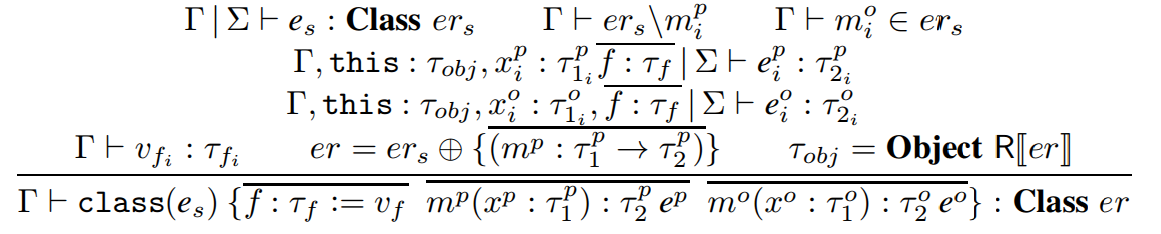
\includegraphics[scale=0.2]{rack_1.png}

	    \tiny Racket
	  \end{column}
	\end{columns}

	\begin{itemize}
		\item Hard to apply to a new language
		\item Key details are completely obscured
		\item Difficult to compare to one another
	\end{itemize}
  \end{frame}
  \begin{frame}{Our mistake}
  	\begin{itemize}
  		\item We understand gradual typing, right?
  		\item Porting some different approaches to one language can't be that hard, surely.
  		\item It can't take that long to do, could be interesting.
  		\item 1 year later ....
  	\end{itemize}
  \end{frame}
  \section{Our Approach}
  \begin{frame}{Calculi}
  \center\begin{minipage}{4cm}\begin{tabular}{l@{~~~}l}
\e &::=  \x \\
   \Alt{ \Get\e\f }
   \Alt{ \Set\e\f\e }
   \Alt{ \Call\e\m{\b\e} }
   \Alt{ \New\C{\b\e} }
   \Alt{ \Cast\t\e }
\end{tabular}\end{minipage}\begin{minipage}{4cm}\begin{tabular}{l@{~~~}l}
\fd &::= 
    \Ftype\f\t   \\
\md &::=
    \Mdef\m\x\t\t\e \\
\c &::= \Class \C {\b{\fd}}{\b{\md} } \\
\mt &::= \Mtype\m{\b\t}\t\\
\t &::= ~ \any \\
   \Alt{ \Type{  \b{ \mt } } }
\end{tabular}\end{minipage}
\end{frame}

\newcommand{\ESub}[3]{#1 \vdash #2 \leq #3}
\begin{frame}{Core System}

\begin{itemize}
\item Gradual typing systems are generally extremely similar, the differences are small.
\item To avoid duplication, we use a common core system.
\item Broadly similar to Gradual Typing for Objects, Siek and Taha 2007.
\item Based on cast insertion, supports structural subtyping, uses the guarded semantics.
\end{itemize}
\end{frame}
\begin{frame}{Static Typing}
\begin{mathpar}
\IRule{W3}{
   \EnvType\E\e\any \\ \b{\EnvType\E{\ep1}\t }
}{
   \EnvType\E{\Call\e\m{\b{\ep1}}}\any
}

\IRule{W4}{
   \EnvType\E\e{\tp1} \\ \Mtype\m{\b{\tp2}}\t\inc \tp1  \\  \b{\EnvType\E{\ep1}{\tp 2}}
}{
    \EnvType\E{\Call\e\m{\b{\ep1}}}\t
} 
\end{mathpar}
\end{frame}
\begin{frame}{Synthetic Cast Insertion}
\begin{mathpar}

\IRule{A4}{
	\GenCast{\E}{\e_1}{\e_2}{\t_1} \\
	\Mtype\m{\b{\tp 2}}{\tp 3} \inc \t_1\\
	\b{\AnaCast{\E}{\e_3}{\e_4}{\tp 2}} \\
}{
	\GenCast{\E}{\Call{\e_1}\m{\b{\e_2}}}{\Call{\e_3}{\m}{\b{\e_4}}}{\tp 3}
}

\IRule{A5}{
	\GenCast{\E}{\e_1}{\e_3}{\any} \\
	\b{\AnaCast{\E}{\e_2}{\e_4}{\any}} \\
}{
	\GenCast{\E}{\Call{\e_1}\m{\b{\e_2}}}{\Call{\Cast{\Type{\Mtype{\Dyn\m}{\b{\any}}\any}}{\e_3}}{\Dyn\m}{\b{\e_4}}}{\any}
}
\end{mathpar}
\centering
\end{frame}
\begin{frame}{Analytic Cast Insertion}
\centering Typically a function of the specific system in question.
\begin{mathpar}
\IRule{AA1}{\GenCast{\E}{\ep1}{\ep2}{\tp 2} \\  {\tp2} \Sub {\tp1}}{\AnaCast\E{\ep1}{\ep2}{\tp1}}

\IRule{AA2}{\GenCast{\E}{\ep1}{\ep2}{\any}}{\AnaCast\E{\ep1}{{\Cast{\tp1}{\ep2}}}{\tp1}}
\end{mathpar}
\centering
\end{frame}
\begin{frame}{Class Translation}
\begin{itemize}
\item For every field $\f:\t$, add getter and setter methods $\f() : \t$ and $\f!(\t):\t$
\item For every method $\m(\b{\t}):\t$ (including getters and setters), add a guard method $\Dyn\m(\b{\any}):\any$, that casts the inputs to the fully specified type and the output to $\any$.
\end{itemize}
\end{frame}
\section{Strongscript}
\begin{frame}{Types}
Strongscript provides programmer control over the soundness guarantee.

It adds a weak type
\[
\t ::= \ldots \B \Weak{\{\b{\mt}\}}
\]

Uses of this type are not strictly checked!
\end{frame}
\begin{frame}{Statics}
\begin{mathpar}
\IRule{STS1}{
}{
	\tp1 \Sub \Weak\tp1
}

\IRule{STS2}{
	\tp1 \Sub \tp2
}{
	\Weak\tp1 \Sub \Weak\tp2
}

\IRule{A5}{
	\GenCast{\E}{\e_1}{\e_1'}{\Weak\tp1} \\
	\b{\AnaCast{\E}{\e_2}{\e_2'}{\any}} \\
}{
	\GenCast{\E}{\Call{\e_1}\m{\b{\e_2}}}{\Call{\e_1'}{\Dyn\m}{\b{\e_2'}}}{\any}
}

\IRule{AASC1}{
	\GenCast{\E}{\ep1}{\ep2}{\Weak\tp2}
}{
	\AnaCast{\E}{\ep1}{\Cast{\tp1}{\ep2}}{\tp1}
}
\end{mathpar}
\end{frame}
\section{Typed Racket}
\begin{frame}{Statics}
Same types as the base, new type checking.

We model module typing by requiring that a class be either fully untyped (no typed field or method declarations) or fully typed.

Typed code is restricted from creating new instances of untyped classes.
\end{frame}
\begin{frame}
Cast insertion is now only ran on the untyped code. 

\end{frame}
\end{document}